% Options for packages loaded elsewhere
\PassOptionsToPackage{unicode}{hyperref}
\PassOptionsToPackage{hyphens}{url}
%
\documentclass[
]{article}
\usepackage{lmodern}
\usepackage{amssymb,amsmath}
\usepackage{ifxetex,ifluatex}
\ifnum 0\ifxetex 1\fi\ifluatex 1\fi=0 % if pdftex
  \usepackage[T1]{fontenc}
  \usepackage[utf8]{inputenc}
  \usepackage{textcomp} % provide euro and other symbols
\else % if luatex or xetex
  \usepackage{unicode-math}
  \defaultfontfeatures{Scale=MatchLowercase}
  \defaultfontfeatures[\rmfamily]{Ligatures=TeX,Scale=1}
\fi
% Use upquote if available, for straight quotes in verbatim environments
\IfFileExists{upquote.sty}{\usepackage{upquote}}{}
\IfFileExists{microtype.sty}{% use microtype if available
  \usepackage[]{microtype}
  \UseMicrotypeSet[protrusion]{basicmath} % disable protrusion for tt fonts
}{}
\makeatletter
\@ifundefined{KOMAClassName}{% if non-KOMA class
  \IfFileExists{parskip.sty}{%
    \usepackage{parskip}
  }{% else
    \setlength{\parindent}{0pt}
    \setlength{\parskip}{6pt plus 2pt minus 1pt}}
}{% if KOMA class
  \KOMAoptions{parskip=half}}
\makeatother
\usepackage{xcolor}
\IfFileExists{xurl.sty}{\usepackage{xurl}}{} % add URL line breaks if available
\IfFileExists{bookmark.sty}{\usepackage{bookmark}}{\usepackage{hyperref}}
\hypersetup{
  pdftitle={Respuestas Examen \#1 IO},
  hidelinks,
  pdfcreator={LaTeX via pandoc}}
\urlstyle{same} % disable monospaced font for URLs
\usepackage[margin=1in]{geometry}
\usepackage{color}
\usepackage{fancyvrb}
\newcommand{\VerbBar}{|}
\newcommand{\VERB}{\Verb[commandchars=\\\{\}]}
\DefineVerbatimEnvironment{Highlighting}{Verbatim}{commandchars=\\\{\}}
% Add ',fontsize=\small' for more characters per line
\usepackage{framed}
\definecolor{shadecolor}{RGB}{248,248,248}
\newenvironment{Shaded}{\begin{snugshade}}{\end{snugshade}}
\newcommand{\AlertTok}[1]{\textcolor[rgb]{0.94,0.16,0.16}{#1}}
\newcommand{\AnnotationTok}[1]{\textcolor[rgb]{0.56,0.35,0.01}{\textbf{\textit{#1}}}}
\newcommand{\AttributeTok}[1]{\textcolor[rgb]{0.77,0.63,0.00}{#1}}
\newcommand{\BaseNTok}[1]{\textcolor[rgb]{0.00,0.00,0.81}{#1}}
\newcommand{\BuiltInTok}[1]{#1}
\newcommand{\CharTok}[1]{\textcolor[rgb]{0.31,0.60,0.02}{#1}}
\newcommand{\CommentTok}[1]{\textcolor[rgb]{0.56,0.35,0.01}{\textit{#1}}}
\newcommand{\CommentVarTok}[1]{\textcolor[rgb]{0.56,0.35,0.01}{\textbf{\textit{#1}}}}
\newcommand{\ConstantTok}[1]{\textcolor[rgb]{0.00,0.00,0.00}{#1}}
\newcommand{\ControlFlowTok}[1]{\textcolor[rgb]{0.13,0.29,0.53}{\textbf{#1}}}
\newcommand{\DataTypeTok}[1]{\textcolor[rgb]{0.13,0.29,0.53}{#1}}
\newcommand{\DecValTok}[1]{\textcolor[rgb]{0.00,0.00,0.81}{#1}}
\newcommand{\DocumentationTok}[1]{\textcolor[rgb]{0.56,0.35,0.01}{\textbf{\textit{#1}}}}
\newcommand{\ErrorTok}[1]{\textcolor[rgb]{0.64,0.00,0.00}{\textbf{#1}}}
\newcommand{\ExtensionTok}[1]{#1}
\newcommand{\FloatTok}[1]{\textcolor[rgb]{0.00,0.00,0.81}{#1}}
\newcommand{\FunctionTok}[1]{\textcolor[rgb]{0.00,0.00,0.00}{#1}}
\newcommand{\ImportTok}[1]{#1}
\newcommand{\InformationTok}[1]{\textcolor[rgb]{0.56,0.35,0.01}{\textbf{\textit{#1}}}}
\newcommand{\KeywordTok}[1]{\textcolor[rgb]{0.13,0.29,0.53}{\textbf{#1}}}
\newcommand{\NormalTok}[1]{#1}
\newcommand{\OperatorTok}[1]{\textcolor[rgb]{0.81,0.36,0.00}{\textbf{#1}}}
\newcommand{\OtherTok}[1]{\textcolor[rgb]{0.56,0.35,0.01}{#1}}
\newcommand{\PreprocessorTok}[1]{\textcolor[rgb]{0.56,0.35,0.01}{\textit{#1}}}
\newcommand{\RegionMarkerTok}[1]{#1}
\newcommand{\SpecialCharTok}[1]{\textcolor[rgb]{0.00,0.00,0.00}{#1}}
\newcommand{\SpecialStringTok}[1]{\textcolor[rgb]{0.31,0.60,0.02}{#1}}
\newcommand{\StringTok}[1]{\textcolor[rgb]{0.31,0.60,0.02}{#1}}
\newcommand{\VariableTok}[1]{\textcolor[rgb]{0.00,0.00,0.00}{#1}}
\newcommand{\VerbatimStringTok}[1]{\textcolor[rgb]{0.31,0.60,0.02}{#1}}
\newcommand{\WarningTok}[1]{\textcolor[rgb]{0.56,0.35,0.01}{\textbf{\textit{#1}}}}
\usepackage{longtable,booktabs}
% Correct order of tables after \paragraph or \subparagraph
\usepackage{etoolbox}
\makeatletter
\patchcmd\longtable{\par}{\if@noskipsec\mbox{}\fi\par}{}{}
\makeatother
% Allow footnotes in longtable head/foot
\IfFileExists{footnotehyper.sty}{\usepackage{footnotehyper}}{\usepackage{footnote}}
\makesavenoteenv{longtable}
\usepackage{graphicx,grffile}
\makeatletter
\def\maxwidth{\ifdim\Gin@nat@width>\linewidth\linewidth\else\Gin@nat@width\fi}
\def\maxheight{\ifdim\Gin@nat@height>\textheight\textheight\else\Gin@nat@height\fi}
\makeatother
% Scale images if necessary, so that they will not overflow the page
% margins by default, and it is still possible to overwrite the defaults
% using explicit options in \includegraphics[width, height, ...]{}
\setkeys{Gin}{width=\maxwidth,height=\maxheight,keepaspectratio}
% Set default figure placement to htbp
\makeatletter
\def\fps@figure{htbp}
\makeatother
\setlength{\emergencystretch}{3em} % prevent overfull lines
\providecommand{\tightlist}{%
  \setlength{\itemsep}{0pt}\setlength{\parskip}{0pt}}
\setcounter{secnumdepth}{-\maxdimen} % remove section numbering

\title{Respuestas Examen \#1 IO}
\author{}
\date{\vspace{-2.5em}}

\begin{document}
\maketitle

\hypertarget{estudiantes}{%
\subsubsection{Estudiantes}\label{estudiantes}}

Randald Villegas Brenes\\
Kevin Andrés Solano Jiménez

\hypertarget{librerias}{%
\subsubsection{Librerias}\label{librerias}}

Librería utilizada en el examen.

\begin{Shaded}
\begin{Highlighting}[]
\KeywordTok{library}\NormalTok{ (lpSolve)}
\end{Highlighting}
\end{Shaded}

\hypertarget{problema-1}{%
\section{Problema \#1}\label{problema-1}}

\hypertarget{tabla-resumen}{%
\subsection{Tabla Resumen}\label{tabla-resumen}}

\begin{figure}
\centering
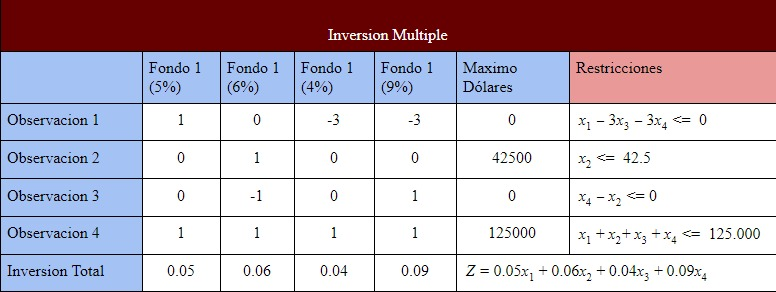
\includegraphics{s1.jpeg}
\caption{``Tabla de resumen''}
\end{figure}

\hypertarget{modelo-de-programaciuxf3n-lineal}{%
\subsection{\texorpdfstring{\textbf{Modelo de programación
lineal}}{Modelo de programación lineal}}\label{modelo-de-programaciuxf3n-lineal}}

\begin{longtable}[]{@{}ll@{}}
\toprule
\endhead
FO: & \(Z=0.05x_1+0.06x_2+0.04x_3+0.09x4\)\tabularnewline
Sujeto a:\(\hspace{1cm}\) & \(x_1-3x_3-3x_4<= 0\)\tabularnewline
& \(x_2<= 42500\)\tabularnewline
& \(x_4-x_2<=0\)\tabularnewline
& \(x_1+x_2+x_3+x_4<= 125.000\)\tabularnewline
\bottomrule
\end{longtable}

\hypertarget{soluciuxf3n-original}{%
\subsection{Solución Original}\label{soluciuxf3n-original}}

\begin{Shaded}
\begin{Highlighting}[]
\CommentTok{# Definición de los coeficientes}
\NormalTok{coef.obj <-}\StringTok{ }\KeywordTok{c}\NormalTok{(}\FloatTok{0.05}\NormalTok{, }\FloatTok{0.06}\NormalTok{, }\FloatTok{0.04}\NormalTok{, }\FloatTok{0.09}\NormalTok{)}

\CommentTok{# Definición de las restricciones}
\NormalTok{coef.restr <-}\StringTok{ }\KeywordTok{matrix}\NormalTok{(}\KeywordTok{c}\NormalTok{(}\DecValTok{1}\NormalTok{, }\DecValTok{0}\NormalTok{, }\DecValTok{-3}\NormalTok{, }\DecValTok{-3}\NormalTok{, }\DecValTok{0}\NormalTok{, }\DecValTok{1}\NormalTok{, }\DecValTok{0}\NormalTok{, }\DecValTok{0}\NormalTok{, }\DecValTok{0}\NormalTok{, }\DecValTok{-1}\NormalTok{, }\DecValTok{0}\NormalTok{, }\DecValTok{1}\NormalTok{, }\DecValTok{1}\NormalTok{, }\DecValTok{1}\NormalTok{, }\DecValTok{1}\NormalTok{, }\DecValTok{1}\NormalTok{), }\DataTypeTok{nrow =} \DecValTok{4}\NormalTok{, }\DataTypeTok{byrow =}\NormalTok{ T)}
\NormalTok{dir.rest <-}\StringTok{ }\KeywordTok{c}\NormalTok{(}\StringTok{"<="}\NormalTok{, }\StringTok{"<="}\NormalTok{, }\StringTok{"<="}\NormalTok{, }\StringTok{"<="}\NormalTok{)}
\NormalTok{param.rest <-}\StringTok{ }\KeywordTok{c}\NormalTok{(}\DecValTok{0}\NormalTok{, }\DecValTok{42500}\NormalTok{, }\DecValTok{0}\NormalTok{, }\DecValTok{125000}\NormalTok{)}

\CommentTok{#Solución del problema}
\NormalTok{solucion <-}\StringTok{ }\KeywordTok{lp}\NormalTok{(}\StringTok{"max"}\NormalTok{, coef.obj, coef.restr, dir.rest, param.rest, }\DataTypeTok{compute.sens =}\NormalTok{ T)}
\end{Highlighting}
\end{Shaded}

\hypertarget{monto-muxe1ximo-de-rendimiento}{%
\subparagraph{Monto Máximo de
rendimiento}\label{monto-muxe1ximo-de-rendimiento}}

\begin{Shaded}
\begin{Highlighting}[]
\NormalTok{solucion}\OperatorTok{$}\NormalTok{objval}
\end{Highlighting}
\end{Shaded}

\begin{verbatim}
## [1] 8375
\end{verbatim}

\begin{Shaded}
\begin{Highlighting}[]
\CommentTok{# El monto máximo es de $8.375}
\end{Highlighting}
\end{Shaded}

\hypertarget{distribuciuxf3n-de-los-125.000}{%
\subparagraph{Distribución de los
\$125.000}\label{distribuciuxf3n-de-los-125.000}}

\begin{Shaded}
\begin{Highlighting}[]
\NormalTok{solucion}\OperatorTok{$}\NormalTok{solution}
\end{Highlighting}
\end{Shaded}

\begin{verbatim}
## [1] 40000 42500     0 42500
\end{verbatim}

\begin{Shaded}
\begin{Highlighting}[]
\CommentTok{# x_1 (Fondo 5%) = $40.000}
\CommentTok{# x_2 (Fondo 6%) = $42.500}
\CommentTok{# x_3 (Fondo 4%) = $0}
\CommentTok{# x_4 (Fondo 9%) = $42.500}
\end{Highlighting}
\end{Shaded}

\hypertarget{punto-4}{%
\subsection{Punto 4}\label{punto-4}}

En este caso los valores o coeficientes de las FO hacen referencias a
los diferentes porcentajes de inverción que se desea realizar en los 4
fondos con respecto a los valores mínimos o máximos de los coeficientes
de la función objetivo, sería los siguientes:

\textbf{Coeficiente 1:} Valor Original: 0.05 ------ Valor Mínimo: 0.04
------ Valor Máximo: 0.075\\
\textbf{Coeficiente 2:} Valor Original: 0.06 ------ Valor Mínimo: 0.01
------ Valor Máximo: Infinito\\
\textbf{Coeficiente 3:} Valor Original: 0.04 ------ Valor Mínimo: 0.04 -
1E+30 ------ Valor Máximo: 0.05\\
\textbf{Coeficiente 4:} Valor Original: 0.09 ------ Valor Mínimo: 0.05
------ Valor Máximo: Infinito

\hypertarget{punto-5}{%
\subsection{Punto 5}\label{punto-5}}

Dentro de las recomendaciones que le daríamos al inversioniste, sería
que a las inversion del 5\%, la aumente a un 7.5\% y las inversiones del
6\% y 9\%, las lleve al 100\% para así obtener una mayor ganancia, esta
recomendacion representaria un gran aumento en las ganacias desde
\textbf{\$8.375} como valor de ganancias gasta \textbf{\$88.000}

\hypertarget{punto-6}{%
\subsection{Punto 6}\label{punto-6}}

Considerando los precios sombra, se recomienda eliminar el valor derecho
0 de la tercera restricción (x\_4 - x\_2 \textless{} 0) y aumentarlo a
lo maximo posible que serían \textbf{\$40.000}, todo esto con base a los
valores sombra

\hypertarget{soluciuxf3n-sugerida-por-analistas-una-vez-aplicado-lo-dicho-en-el-punto-5-y-6}{%
\paragraph{Solución Sugerida por analistas una vez aplicado lo dicho en
el Punto 5 y
6}\label{soluciuxf3n-sugerida-por-analistas-una-vez-aplicado-lo-dicho-en-el-punto-5-y-6}}

\begin{Shaded}
\begin{Highlighting}[]
\CommentTok{# Definición de los coeficientes}
\NormalTok{coef.obj <-}\StringTok{ }\KeywordTok{c}\NormalTok{(}\FloatTok{0.075}\NormalTok{, }\DecValTok{1}\NormalTok{, }\FloatTok{0.00}\NormalTok{, }\DecValTok{1}\NormalTok{)}

\CommentTok{# Definición de las restricciones}
\NormalTok{coef.restr <-}\StringTok{ }\KeywordTok{matrix}\NormalTok{(}\KeywordTok{c}\NormalTok{(}\DecValTok{1}\NormalTok{, }\DecValTok{0}\NormalTok{, }\DecValTok{-3}\NormalTok{, }\DecValTok{-3}\NormalTok{, }\DecValTok{0}\NormalTok{, }\DecValTok{1}\NormalTok{, }\DecValTok{0}\NormalTok{, }\DecValTok{0}\NormalTok{, }\DecValTok{0}\NormalTok{, }\DecValTok{-1}\NormalTok{, }\DecValTok{0}\NormalTok{, }\DecValTok{1}\NormalTok{, }\DecValTok{1}\NormalTok{, }\DecValTok{1}\NormalTok{, }\DecValTok{1}\NormalTok{, }\DecValTok{1}\NormalTok{), }\DataTypeTok{nrow =} \DecValTok{4}\NormalTok{, }\DataTypeTok{byrow =}\NormalTok{ T)}
\NormalTok{dir.rest <-}\StringTok{ }\KeywordTok{c}\NormalTok{(}\StringTok{"<="}\NormalTok{, }\StringTok{"<="}\NormalTok{, }\StringTok{"<="}\NormalTok{, }\StringTok{"<="}\NormalTok{)}
\NormalTok{param.rest <-}\StringTok{ }\KeywordTok{c}\NormalTok{(}\DecValTok{0}\NormalTok{, }\DecValTok{42500}\NormalTok{, }\DecValTok{40000}\NormalTok{, }\DecValTok{125000}\NormalTok{)}

\CommentTok{#Solución del problema}
\NormalTok{solucion1 <-}\StringTok{ }\KeywordTok{lp}\NormalTok{(}\StringTok{"max"}\NormalTok{, coef.obj, coef.restr, dir.rest, param.rest, }\DataTypeTok{compute.sens =}\NormalTok{ T)}
\end{Highlighting}
\end{Shaded}

\hypertarget{monto-muxe1ximo-de-rendimiento-1}{%
\subparagraph{Monto Máximo de
rendimiento}\label{monto-muxe1ximo-de-rendimiento-1}}

\begin{Shaded}
\begin{Highlighting}[]
\NormalTok{solucion1}\OperatorTok{$}\NormalTok{objval}
\end{Highlighting}
\end{Shaded}

\begin{verbatim}
## [1] 125000
\end{verbatim}

\begin{Shaded}
\begin{Highlighting}[]
\CommentTok{# El monto máximo es de $125.000}
\end{Highlighting}
\end{Shaded}

\hypertarget{distribuciuxf3n-de-los-125.000-1}{%
\subparagraph{Distribución de los
\$125.000}\label{distribuciuxf3n-de-los-125.000-1}}

\begin{Shaded}
\begin{Highlighting}[]
\NormalTok{solucion1}\OperatorTok{$}\NormalTok{solution}
\end{Highlighting}
\end{Shaded}

\begin{verbatim}
## [1]     0 42500     0 82500
\end{verbatim}

\begin{Shaded}
\begin{Highlighting}[]
\CommentTok{# x_1 (Fondo 5%) = $0}
\CommentTok{# x_2 (Fondo 6%) = $42.500}
\CommentTok{# x_3 (Fondo 4%) = $0}
\CommentTok{# x_4 (Fondo 9%) = $82.500}
\end{Highlighting}
\end{Shaded}

\hypertarget{problema-2}{%
\section{Problema \#2}\label{problema-2}}

\hypertarget{tabla-de-resumen}{%
\subsection{Tabla de resumen}\label{tabla-de-resumen}}

\hypertarget{la-siguiente-tabla-se-utilizo-para-representar-la-combinacion-de-variables-de-las-comunidades-y-las-cosechas-con-el-proposito-de-representar-de-una-manera-mas-legible-el-problema-con-la-herramienta-de-solver}{%
\paragraph{La siguiente tabla se utilizo para representar la combinacion
de variables de las comunidades y las cosechas, con el proposito de
representar de una manera mas legible el problema con la herramienta de
solver:}\label{la-siguiente-tabla-se-utilizo-para-representar-la-combinacion-de-variables-de-las-comunidades-y-las-cosechas-con-el-proposito-de-representar-de-una-manera-mas-legible-el-problema-con-la-herramienta-de-solver}}

\begin{figure}
\centering
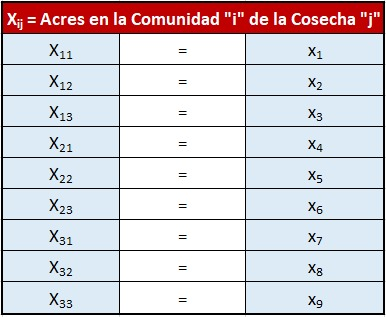
\includegraphics{symbols.jpeg}
\caption{``Tabla de simbolos utilizada para representar las variables
que se mezclan en el problema''}
\end{figure}

\hypertarget{despues-de-plantear-las-combinacion-de-las-variables-se-procede-a-organizar-los-datos-que-brinda-el-problema}{%
\paragraph{Despues de plantear las combinacion de las variables, se
procede a organizar los datos que brinda el
problema:}\label{despues-de-plantear-las-combinacion-de-las-variables-se-procede-a-organizar-los-datos-que-brinda-el-problema}}

\begin{figure}
\centering
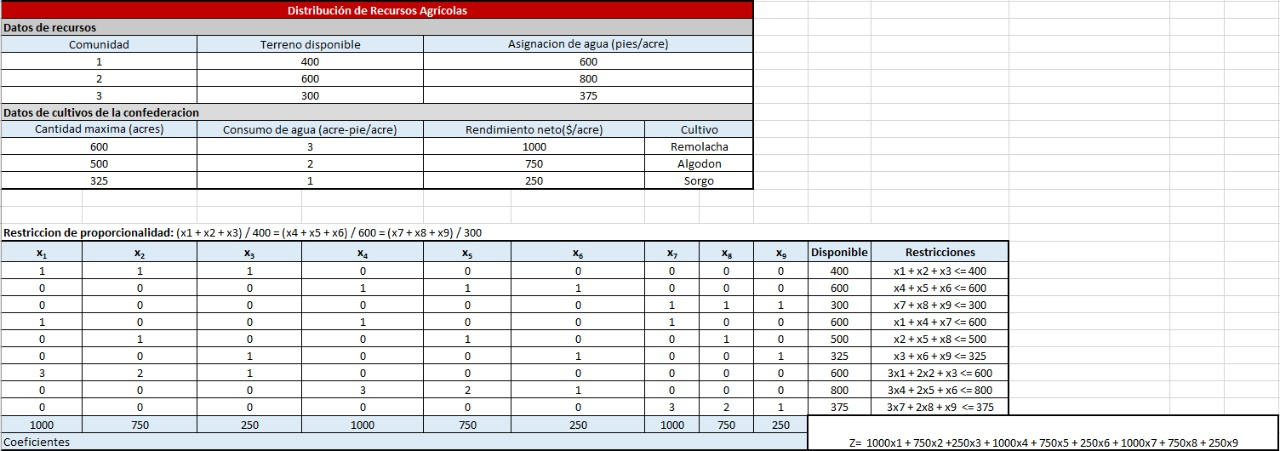
\includegraphics{img1.jpeg}
\caption{``Tabla de resumen utilizada para plantear el problema''}
\end{figure}

\hypertarget{modelo-de-programaciuxf3n-lineal-1}{%
\subsection{Modelo de programación
lineal}\label{modelo-de-programaciuxf3n-lineal-1}}

\begin{itemize}
\item
  Función Objetivo: \textbf{(Maximizar)} Z = 1000(x1 + x4 +x7) + 750(x2
  + x5 + x8) + 250(x3 + x6 + x9)
\item
  Z= 1000x1 + 750x2 +250x3 + 1000x4 + 750x5 + 250x6 + 1000x7 + 750x8 +
  250x9
\end{itemize}

\hypertarget{restricciones}{%
\subsubsection{Restricciones:}\label{restricciones}}

\hypertarget{primero-se-delimita-la-cantidad-de-terreno-disponible-para-cada-una-de-las-comunidades}{%
\paragraph{Primero se delimita la cantidad de terreno disponible para
cada una de las
comunidades:}\label{primero-se-delimita-la-cantidad-de-terreno-disponible-para-cada-una-de-las-comunidades}}

\begin{itemize}
\tightlist
\item
  \textbf{x1 + x2 + x3 \textless= 400}
\item
  \textbf{x4 + x5 + x6 \textless= 600}
\item
  \textbf{x7 + x8 + x9 \textless= 300}
\end{itemize}

\hypertarget{luego-se-delimita-la-cantidad-de-terreno-disponible-para-cada-una-de-las-cosechas-disponibles}{%
\paragraph{Luego se delimita la cantidad de terreno disponible para cada
una de las cosechas
disponibles:}\label{luego-se-delimita-la-cantidad-de-terreno-disponible-para-cada-una-de-las-cosechas-disponibles}}

\begin{itemize}
\tightlist
\item
  \textbf{x1 + x4 + x7 \textless= 600}
\item
  \textbf{x2 + x5 + x8 \textless= 500}
\item
  \textbf{x3 + x6 + x9 \textless= 325}
\end{itemize}

\hypertarget{seguidamente-se-delimita-la-cantidad-de-agua-disponible-para-cada-una-de-las-comunidades}{%
\paragraph{Seguidamente se delimita la cantidad de agua disponible para
cada una de las
comunidades:}\label{seguidamente-se-delimita-la-cantidad-de-agua-disponible-para-cada-una-de-las-comunidades}}

\begin{itemize}
\tightlist
\item
  \textbf{3x1 + 2x2 + x3 \textless= 600}
\item
  \textbf{3x4 + 2x5 + x6 \textless= 800}
\item
  \textbf{3x7 + 2x8 + x9 \textless= 375}
\end{itemize}

\hypertarget{finalmente-se-agregan-3-restricciones-que-aseguran-que-se-cumpla-que-entre-las-tres-comunidades-se-siembre-la-misma-proporciuxf3n-de-sus-tierras}{%
\paragraph{Finalmente se agregan 3 restricciones que aseguran que se
cumpla que entre las tres comunidades se siembre la misma proporción de
sus
tierras:}\label{finalmente-se-agregan-3-restricciones-que-aseguran-que-se-cumpla-que-entre-las-tres-comunidades-se-siembre-la-misma-proporciuxf3n-de-sus-tierras}}

\begin{itemize}
\tightlist
\item
  \textbf{(x1 + x2 + x3) / 400 = (x4 + x5 + x6) / 600 = (x7 + x8 + x9) /
  300}
\end{itemize}

\hypertarget{problema-planteado-para-resolverlo-con-solver}{%
\subsection{Problema planteado para resolverlo con
Solver}\label{problema-planteado-para-resolverlo-con-solver}}

\begin{figure}
\centering
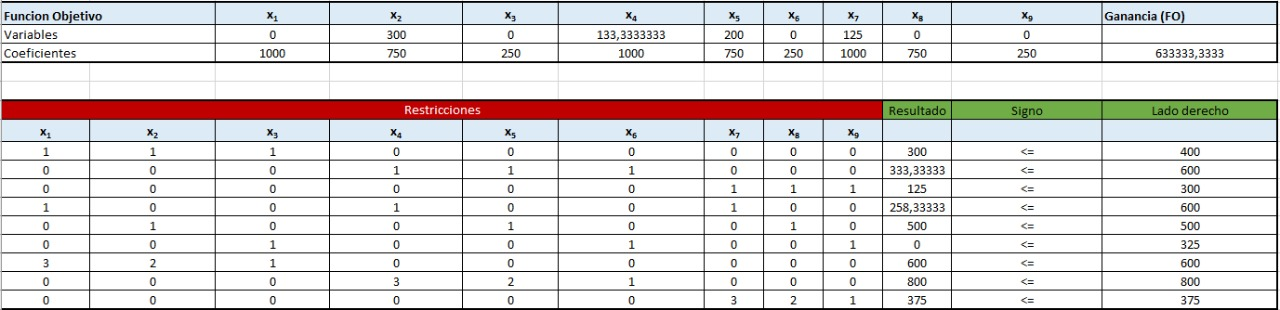
\includegraphics{img2.jpeg}
\caption{``Tabla con restricciones y los resultados que brinda Solver''}
\end{figure}

\hypertarget{la-solucion-optima-que-brinda-solver-es}{%
\paragraph{La solucion optima que brinda Solver
es:}\label{la-solucion-optima-que-brinda-solver-es}}

\begin{itemize}
\tightlist
\item
  \textbf{x1 = 0}
\item
  \textbf{x2 = 300}
\item
  \textbf{x3 = 0}
\item
  \textbf{x4 = 133,3333333}
\item
  \textbf{x5 = 200}
\item
  \textbf{x6 = 0}
\item
  \textbf{x7 = 125}
\item
  \textbf{x8 = 0}
\item
  \textbf{x9 = 0}
\end{itemize}

\hypertarget{con-los-datos-que-brinda-solver-se-puede-interpretar-que-en-la-comunidad-1-se-sembraran-300-acres-de-algodon-en-la-comunidad-2-se-sembraran-133.3333333-de-remolachas-200-de-algodon-y-en-la-comunidad-3-se-sembraran-123-remolachas.}{%
\paragraph{Con los datos que brinda solver, se puede interpretar que en
la comunidad 1, se sembraran 300 acres de algodon, en la comunidad 2, se
sembraran 133.3333333 de remolachas, 200 de algodon y en la comunidad 3
se sembraran 123
remolachas.}\label{con-los-datos-que-brinda-solver-se-puede-interpretar-que-en-la-comunidad-1-se-sembraran-300-acres-de-algodon-en-la-comunidad-2-se-sembraran-133.3333333-de-remolachas-200-de-algodon-y-en-la-comunidad-3-se-sembraran-123-remolachas.}}

\hypertarget{con-la-funciuxf3n-objetivo-con-un-valor-de-6333333333}{%
\paragraph{\texorpdfstring{Con la función objetivo con un valor de
\textbf{633333,3333}}{Con la función objetivo con un valor de 633333,3333}}\label{con-la-funciuxf3n-objetivo-con-un-valor-de-6333333333}}

\hypertarget{entre-los-componentes-de-restricciuxf3n-terreno-agua-cultivo-proporcionalidad-si-hubiese-posibilidad-de-modificar-las-restricciones-se-determina-que-los-que-puede-incidir-muxe1s-en-la-variaciuxf3n-del-rendimiento-total-son}{%
\subsection{Entre los componentes de restricción (terreno, agua,
cultivo, proporcionalidad) si hubiese posibilidad de modificar las
restricciones, se determina que los que puede incidir más en la
variación del rendimiento total
son:}\label{entre-los-componentes-de-restricciuxf3n-terreno-agua-cultivo-proporcionalidad-si-hubiese-posibilidad-de-modificar-las-restricciones-se-determina-que-los-que-puede-incidir-muxe1s-en-la-variaciuxf3n-del-rendimiento-total-son}}

\begin{itemize}
\tightlist
\item
  \textbf{El agua}
\item
  \textbf{El cultivo}
\end{itemize}

\hypertarget{debido-a-que-como-se-menciona-al-inicio-el-principal-problema-es-el-agua-y-eso-implica-que-no-se-pueda-sembrar-muchos-cultivos-lo-que-los-hace-incidir-mas-en-el-rendimiento-total.}{%
\paragraph{Debido a que como se menciona al inicio, el principal
problema es el agua y eso implica que no se pueda sembrar muchos
cultivos, lo que los hace incidir mas en el rendimiento
total.}\label{debido-a-que-como-se-menciona-al-inicio-el-principal-problema-es-el-agua-y-eso-implica-que-no-se-pueda-sembrar-muchos-cultivos-lo-que-los-hace-incidir-mas-en-el-rendimiento-total.}}

\hypertarget{si-la-confederaciuxf3n-consultara-sobre-la-posibilidad-de-aumentar-el-rendimiento-total-pero-partiendo-del-hecho-de-que-no-es-posible-aumentar-la-disponibilidad-de-agua-para-cultivo-quuxe9-le-recomiendaruxedan-modificar-y-cuuxe1l-seruxeda-el-efecto-en-el-rendimiento}{%
\subsection{Si la confederación consultara sobre la posibilidad de
aumentar el rendimiento total, pero partiendo del hecho de que NO es
posible aumentar la disponibilidad de agua para cultivo, ¿qué le
recomiendarían modificar y cuál sería el efecto en el
rendimiento?}\label{si-la-confederaciuxf3n-consultara-sobre-la-posibilidad-de-aumentar-el-rendimiento-total-pero-partiendo-del-hecho-de-que-no-es-posible-aumentar-la-disponibilidad-de-agua-para-cultivo-quuxe9-le-recomiendaruxedan-modificar-y-cuuxe1l-seruxeda-el-efecto-en-el-rendimiento}}

\begin{itemize}
\tightlist
\item
  \textbf{x5}
\item
  \textbf{x7}
\item
  \textbf{x8}
\item
  \textbf{x9}
\end{itemize}

\hypertarget{debido-a-que-segun-el-precio-sombra-que-muestra-en-el-analisis-de-sencibilidad-se-ve-reflejado-el-incremento-que-se-puede-generar-si-se-mantiene-el-los-limites-de-los-permisibles}{%
\paragraph{Debido a que segun el precio sombra que muestra en el
analisis de sencibilidad se ve reflejado el incremento que se puede
generar si se mantiene el los limites de los
permisibles:}\label{debido-a-que-segun-el-precio-sombra-que-muestra-en-el-analisis-de-sencibilidad-se-ve-reflejado-el-incremento-que-se-puede-generar-si-se-mantiene-el-los-limites-de-los-permisibles}}

\begin{figure}
\centering
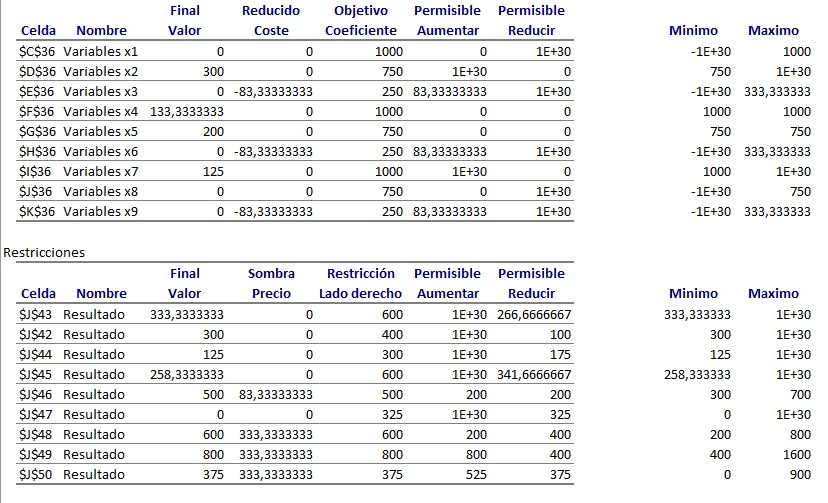
\includegraphics{analisis.jpeg}
\caption{``Tabla analisis de sencibilidad''}
\end{figure}

\hypertarget{cuuxe1l-seruxeda-el-rendimiento-muxe1ximo-esperado.}{%
\subsection{¿Cuál sería el rendimiento máximo
esperado?.}\label{cuuxe1l-seruxeda-el-rendimiento-muxe1ximo-esperado.}}

\hypertarget{el-rendimiento-esperado-es-pasar-de-una-ganancia-de-6333333333-a-1125000-esto-se-nota-gracias-al-analisis-de-sencicilidad-el-cual-muestra-que-los-valores-de-x5-x7-x8-x9-tienen-un-precio-de-sombra-mayor-que-cero-entonces-aumentando-los-valores-del-lado-derecho-de-las-restricciones-y-respetando-el-rango-que-se-puede-maximizar-se-puede-aumentar-el-rendimiento-acontinuacion-se-muestra-una-tabla-con-los-valores-sugeridos-y-su-maximo-rendimiento}{%
\paragraph{\texorpdfstring{El rendimiento esperado es pasar de una
ganancia de \textbf{633333,3333} a \textbf{1125000}, esto se nota
gracias al analisis de sencicilidad el cual muestra que los valores de
x5, x7, x8, x9 tienen un precio de sombra mayor que cero, entonces
aumentando los valores del lado derecho de las restricciones y
respetando el rango que se puede maximizar se puede aumentar el
rendimiento , acontinuacion se muestra una tabla con los valores
sugeridos y su maximo
rendimiento:}{El rendimiento esperado es pasar de una ganancia de 633333,3333 a 1125000, esto se nota gracias al analisis de sencicilidad el cual muestra que los valores de x5, x7, x8, x9 tienen un precio de sombra mayor que cero, entonces aumentando los valores del lado derecho de las restricciones y respetando el rango que se puede maximizar se puede aumentar el rendimiento , acontinuacion se muestra una tabla con los valores sugeridos y su maximo rendimiento:}}\label{el-rendimiento-esperado-es-pasar-de-una-ganancia-de-6333333333-a-1125000-esto-se-nota-gracias-al-analisis-de-sencicilidad-el-cual-muestra-que-los-valores-de-x5-x7-x8-x9-tienen-un-precio-de-sombra-mayor-que-cero-entonces-aumentando-los-valores-del-lado-derecho-de-las-restricciones-y-respetando-el-rango-que-se-puede-maximizar-se-puede-aumentar-el-rendimiento-acontinuacion-se-muestra-una-tabla-con-los-valores-sugeridos-y-su-maximo-rendimiento}}

\begin{figure}
\centering
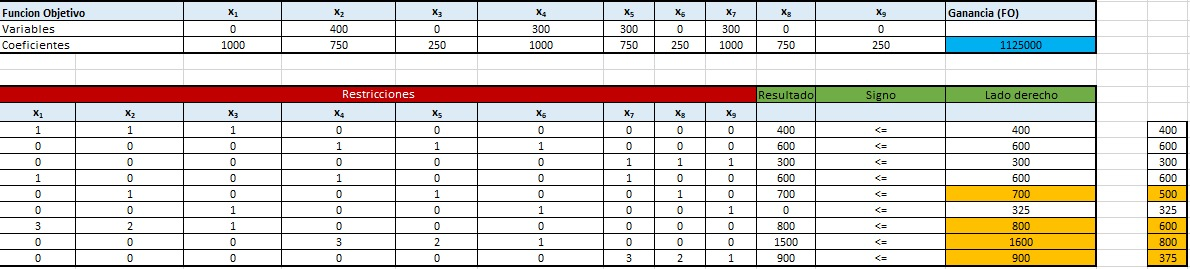
\includegraphics{max.jpeg}
\caption{``Tabla aumento de rendimiento''}
\end{figure}

\end{document}
